% ---------
%  Compile with "pdflatex hw0".
% --------
%!TEX TS-program = pdflatex
%!TEX encoding = UTF-8 Unicode

\documentclass[11pt]{article}
\usepackage{jeffe,handout,graphicx}
\usepackage[utf8]{inputenc}		% Allow some non-ASCII Unicode in source

%  Redefine suits
\usepackage{pifont}
\def\Spade{\text{\ding{171}}}
\def\Heart{\text{\textcolor{Red}{\ding{170}}}}
\def\Diamond{\text{\textcolor{Red}{\ding{169}}}}
\def\Club{\text{\ding{168}}}

\def\Cdot{\mathbin{\text{\normalfont \textbullet}}}
\def\Sym#1{\textbf{\texttt{\color{BrickRed}#1}}}
\newcommand{\comp}[1]{#1_{\text{comp}}}

\newtheorem{Lemma}{lemma}

\usepackage{tikz}
\usetikzlibrary{automata, positioning}

% =====================================================
%   Define common stuff for solution headers
% =====================================================
\Class{CS/ECE 374}
\Semester{Spring 2017}
\Authors{2}
\AuthorOne{Lanxiao Bai}{lbai5}
\AuthorTwo{Renheng Ruan}{rruan2}
%\Section{}

% =====================================================
\begin{document}

% ---------------------------------------------------------


\HomeworkHeader{2}{1}	% homework number, problem number

\begin{quote}
\begin{enumerate}
\item Draw an NFA that accepts the language $\{w \mid$ there is exactly one  block of $0$s of even length\}.  (A ``block of $0$s'' is a maximal substring of $0$s.)
\item 
\begin{enumerate}
\item Draw an NFA for the regular expression $(010)^* + (01)^* + 0^*.$
\item Now using the powerset construction (also called the subset construcion), design a DFA for the same language.  Label the states of your DFA with names that are sets of states of your NFA.
\end{enumerate}
\end{enumerate}
\end{quote}
\hrule

\begin{solution}
	\begin{enumerate}
		\item The NFA is as presented bellow:
			\begin{figure}[h]
				\begin{center}
					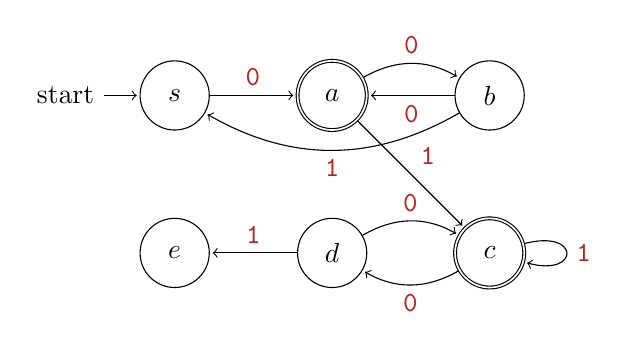
\begin{tikzpicture}[shorten >=1pt,node distance=2cm,on grid,auto]
						\node[state, initial] (s) {$s$};
						\node[state, accepting] (a) [right of=s] {$a$};
						\node[state] (b) [right of =a] {$b$};
						\node[state, accepting] (c) [below of=b] {$c$};
						\node[state] (d) [left of=c] {$d$};
						\node[state] (e) [left of=d] {$e$};
						\path[->]
						(s) edge node {\Sym0} (a)
						(a) edge [bend left] node {\Sym0} (b)
							edge node {\Sym1} (c)
						(b) edge node {\Sym0} (a)
							edge [bend left] node {\Sym1} (s)
						(c) edge [loop right] node {\Sym1} ()
							edge [bend left] node {\Sym0} (d)
						(d) edge [bend left] node {\Sym0} (c)
							edge node [swap] {\Sym1} (e)
						;
					\end{tikzpicture}
					\caption{NFA that accepts \{w $\mid$ there is exactly one  block of $0$s of even length\}}
				\end{center}
			\end{figure}
		\item 
		\begin{enumerate}
			\item 
				Regular expression $(010)^* + (01)^* + 0^*$ accepted by NFA is presented below:
				\begin{figure}[h]
					\begin{center}
						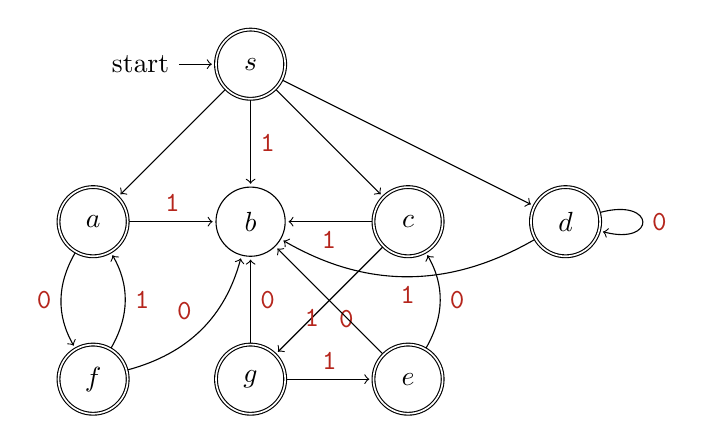
\begin{tikzpicture}[shorten >=1pt,node distance=2cm,on grid,auto]
							\node[state, accepting, initial] (s) {$s$};
							\node[state] (b) [below of=s] {$b$};
							\node[state, accepting] (a) [left of=b] {$a$};
							\node[state, accepting] (c) [right of=b] {$c$};
							\node[state, accepting] (d) [right of=c] {$d$};
							\node[state, accepting] (g) [below of=b] {$g$};
							\node[state, accepting] (f) [left of=g] {$f$};
							\node[state, accepting] (e) [right of=g] {$e$};
							\path[->]
							(s) edge node {\Sym1} (b)
							    edge node {$\e$} (a)
							    edge node {$\e$} (c)
							    edge node {$\e$} (d)
							(a) edge node {\Sym1} (b)
								edge [swap, bend right] node {\Sym0} (f)
							(c) edge node {\Sym1} (b)
								edge node {\Sym0} (g)
						    (d) edge [loop right] node {\Sym0} ()
						    		edge [bend left] node {\Sym1} (b)
						    (f) edge [swap, bend right] node {\Sym1} (a)
						    		edge [bend right] node {\Sym0} (b)
						    	(g) edge [swap] node {\Sym0} (b)
						    		edge node {\Sym1} (e)
						    	(e) edge [swap, bend right] node {\Sym0} (c)
						    		edge node {\Sym1} (b)
							;
						\end{tikzpicture}
						\caption{NFA that accepts $(010)^* + (01)^* + 0^*$}
					\end{center}
				\end{figure}
				\clearpage
			\item Regular expression $(010)^* + (01)^* + 0^*$ accepted by DFA is presented below:
			
			\begin{figure}[h]
					\begin{center}
						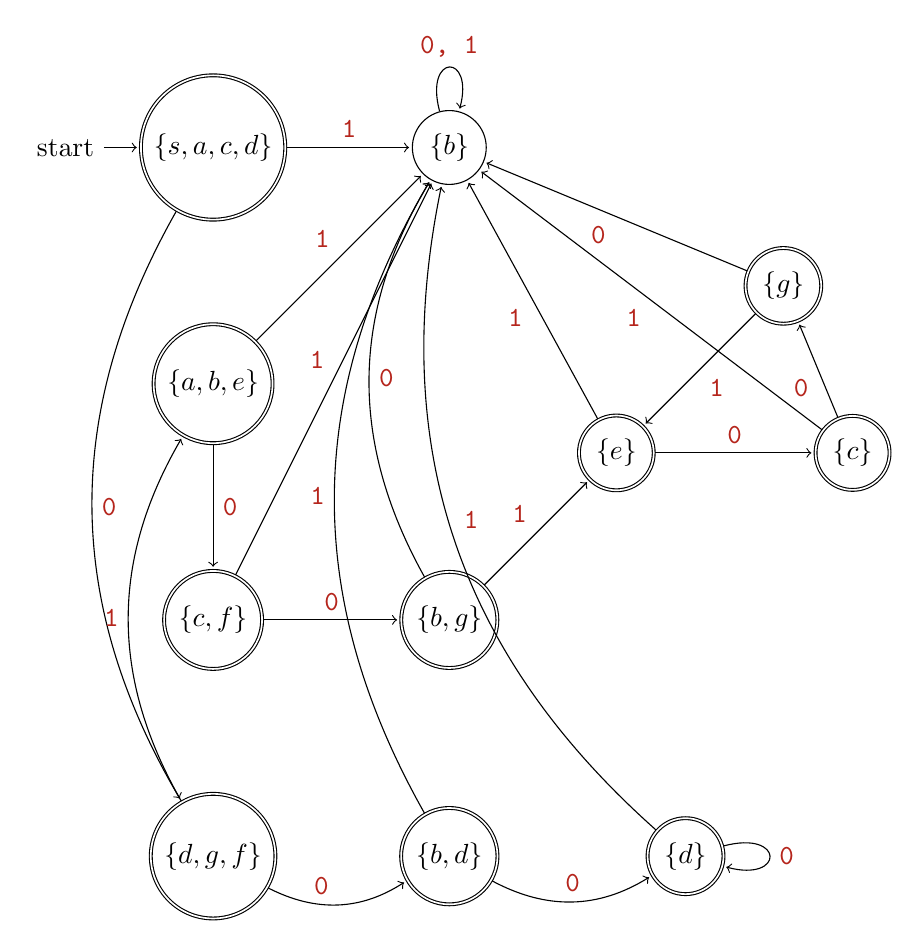
\begin{tikzpicture}[shorten >=1pt,node distance=3cm,on grid,auto]
							\node[state, accepting, initial] (sacd) {$\{s, a, c, d\}$};
							\node[state] (b) [right of=sacd] {$\{b\}$};
							\node[state, accepting] (abe) [below of=sacd] {$\{a, b, e\}$};
							\node[state, accepting] (cf) [below of=abe] {$\{c,f\}$};
							\node[state, accepting] (dgf) [below of=cf] {$\{d,g,f\}$};
							\node[state, accepting] (bd) [right of=dgf] {$\{b, d\}$};
							\node[state, accepting] (d) [right of=bd] {$\{d\}$};
							\node[state, accepting] (bg) [right of=cf] {$\{b, g\}$};
							\node[state, accepting] (e) [above right of=bg] {$\{e\}$};
							\node[state, accepting] (g) [above right of=e] {$\{g\}$};
							\node[state, accepting] (c) [right of=e] {$\{c\}$};
							\path[->]
							(sacd) edge [bend right] node {\Sym0} (dgf)
								   edge node {\Sym1} (b)
							(b) edge [loop above] node {\Sym{0, 1}} ()
							(dgf) edge [bend right] node {\Sym0} (bd)
								  edge [bend left] node {\Sym1} (abe)
							(bd) edge [bend right] node {\Sym0} (d)
								 edge [bend left] node {\Sym1} (b)
							(d) edge [loop right] node {\Sym0} ()
								edge [swap, bend left] node {\Sym1} (b)
							(abe) edge node {\Sym0} (cf)
								  edge node {\Sym1} (b)
							(cf) edge node {\Sym0} (bg)
								 edge node {\Sym1} (b)
							(bg) edge node {\Sym1} (e)
								 edge [swap, bend left] node {\Sym0} (b)
							(e) edge node {\Sym0} (c)
								edge node {\Sym1} (b)
							(c) edge node {\Sym0} (g)
								edge node {\Sym1} (b)
							(g) edge node {\Sym1} (e)
								edge node {\Sym0} (b)
							;
						\end{tikzpicture}
						\caption{DFA that accepts $(010)^* + (01)^* + 0^*$}
					\end{center}
				\end{figure}
		\end{enumerate}
	\end{enumerate}

\end{solution}
\clearpage


% ---------------------------------------------------------
% Change authors for all future solutions
\HomeworkHeader{2}{2}

\begin{quote}
This problem is to illustrate proofs of (the many) closure properties of 
  regular languages.
  \begin{enumerate}
  \item For a language $L$ let
    $\text{FUNKY}(L) = \{w \mid \mbox{$w \in L$ but no proper prefix
    of $w$ is in $L$}\}$. Prove that if $L$ is regular then
    $\text{FUNKY}(L)$ is also regular using the following technique.
    Let $M=(Q,\Sigma,\delta,s,A)$ be a DFA accepting $L$. Describe
    a NFA $N$ in terms of $M$ that accepts $\text{FUNKY}(L)$. Explain
    the construction of your NFA.
  \item In Lab 3 we saw that $\emph{insert}\Sym1(L)$ is regular
    whenever $L$ is regular. Here we consider a different proof technique.
    Let $r$ be a regular expression. We would like to show
    that there is another regular expression $r'$ such that
    $L(r') = \emph{insert}\Sym1(L(r))$. 
    \begin{enumerate}
    \item For each of the base cases of regular expressions
      $\emptyset, \epsilon$ and $\{a\}, a \in \Sigma$ describe
      a regular expression for $\emph{insert}\Sym1(L(r))$.
    \item Suppose $r_1$ and $r_2$ are regular expressions, and
      $r'_1$ and $r'_2$ are regular expressions for the languages
      $\emph{insert}\Sym1(L(r_1))$ and $\emph{insert}\Sym1(L(r_2))$
      respectively. Describe a regular expression for the language
      $\emph{insert}\Sym1(L(r_1+r_2))$ using $r_1,r_2,r'_1,r'_2$.
    \item Same as the previous part but now consider $L(r_1r_2)$.
    \item Same as the previous part but now consider $L((r_1)^*)$.
    \end{enumerate}
  \end{enumerate}
\end{quote}
\hrule


\begin{solution}

\begin{enumerate}
	\item 
		Since $\text{FUNKY}(L)$ contains $w$ that none of it's proper prefix is in $L$, so we can formalize it as
			\[\text{FUNKY}(L) = L - L\Sigma^+\]
		which means that if $a$ is an accepting states in DFA that accepts $L$, for all non-zero length $w$, $\delta(a, w)$ should not be accepted.
		
		As a result, the NSA that accepts $\text{FUNKY}(L)$ is $N = (Q_N, \Sigma_N, \delta_N, s_N, A_N)$ that 
		
		\begin{itemize}
			\item $Q_N = Q$
			\item $\Sigma_N = \Sigma$
			\item $\delta_N: Q \times \Sigma \rightarrow \mathbb{P}(Q)$, that $\delta_N(q, w) = \{\delta(q', w) : q' \in \e\text{reach}(q)\}$
			\item $s_N = s$
			\item $A_N = A - \bigcup_{a \in A, w \in \{w \in L: |w| > 0\}}\delta(a, w)$
		\end{itemize}
		
	\item
		\begin{enumerate}
			\item
				\begin{itemize}
					\item When $r = \emptyset$, $r' = \emptyset$
					\item When $r = \e$, $r = 1$
					\item When $r = a, a \in \Sigma$, $r' = 1r + r1$
				\end{itemize}
			\item For $\emph{insert}\Sym1(L(r_1+r_2))$, $r' = r'_1 + r'_2$
			\item For $\emph{insert}\Sym1(L(r_1r_2))$, $r' = r'_1r_2 + r_1r'_2$
			\item For $\emph{insert}\Sym1(L(r_1)^*)$, $r' = (r_1)^*r'_1(r_1)^*$
		\end{enumerate}
\end{enumerate}


\end{solution}

\end{document}
 